%%%%%%%%%%%%%%%%%%%%%%%%%%%%%%%%%%%%%%%%%%%%%%%%%%%%%%%%%%%%%
%% APPENDICES
%%%%%%%%%%%%%%%%%%%%%%%%%%%%%%%%%%%%%%%%%%%%%%%%%%%%%%%%%%%%%
\appendix

\chapter{Appendix}
\label{app:acronyms}
%% acronyms
\printindex
\printglossaries

%\section{Data sets/Statistical Overview}
%\label{app:data_sets}

\clearpage
\section{MySQL Database}
\label{app:mysql_database}
% image of the mysql database
\begin{figure}[ht]
	\centering
    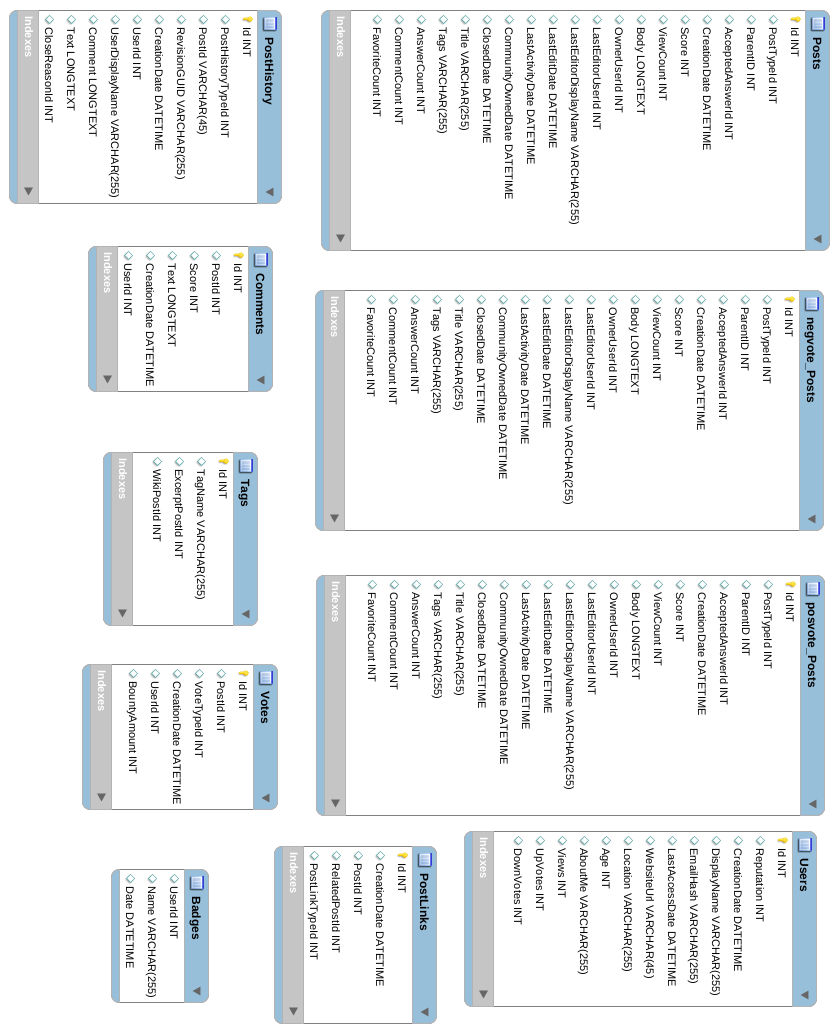
\includegraphics[width=0.8\textwidth]{so_database}
	\caption{MySQL Database used for dataset}
	\label{fig:mysql_database}
\end{figure}

\clearpage
\section{Scikit-learns roadmap - Choosing the right estimator}
\label{app:ml_map}
% image of the cheat-sheet from scikit-learn
\begin{figure}[ht]
	\centering
	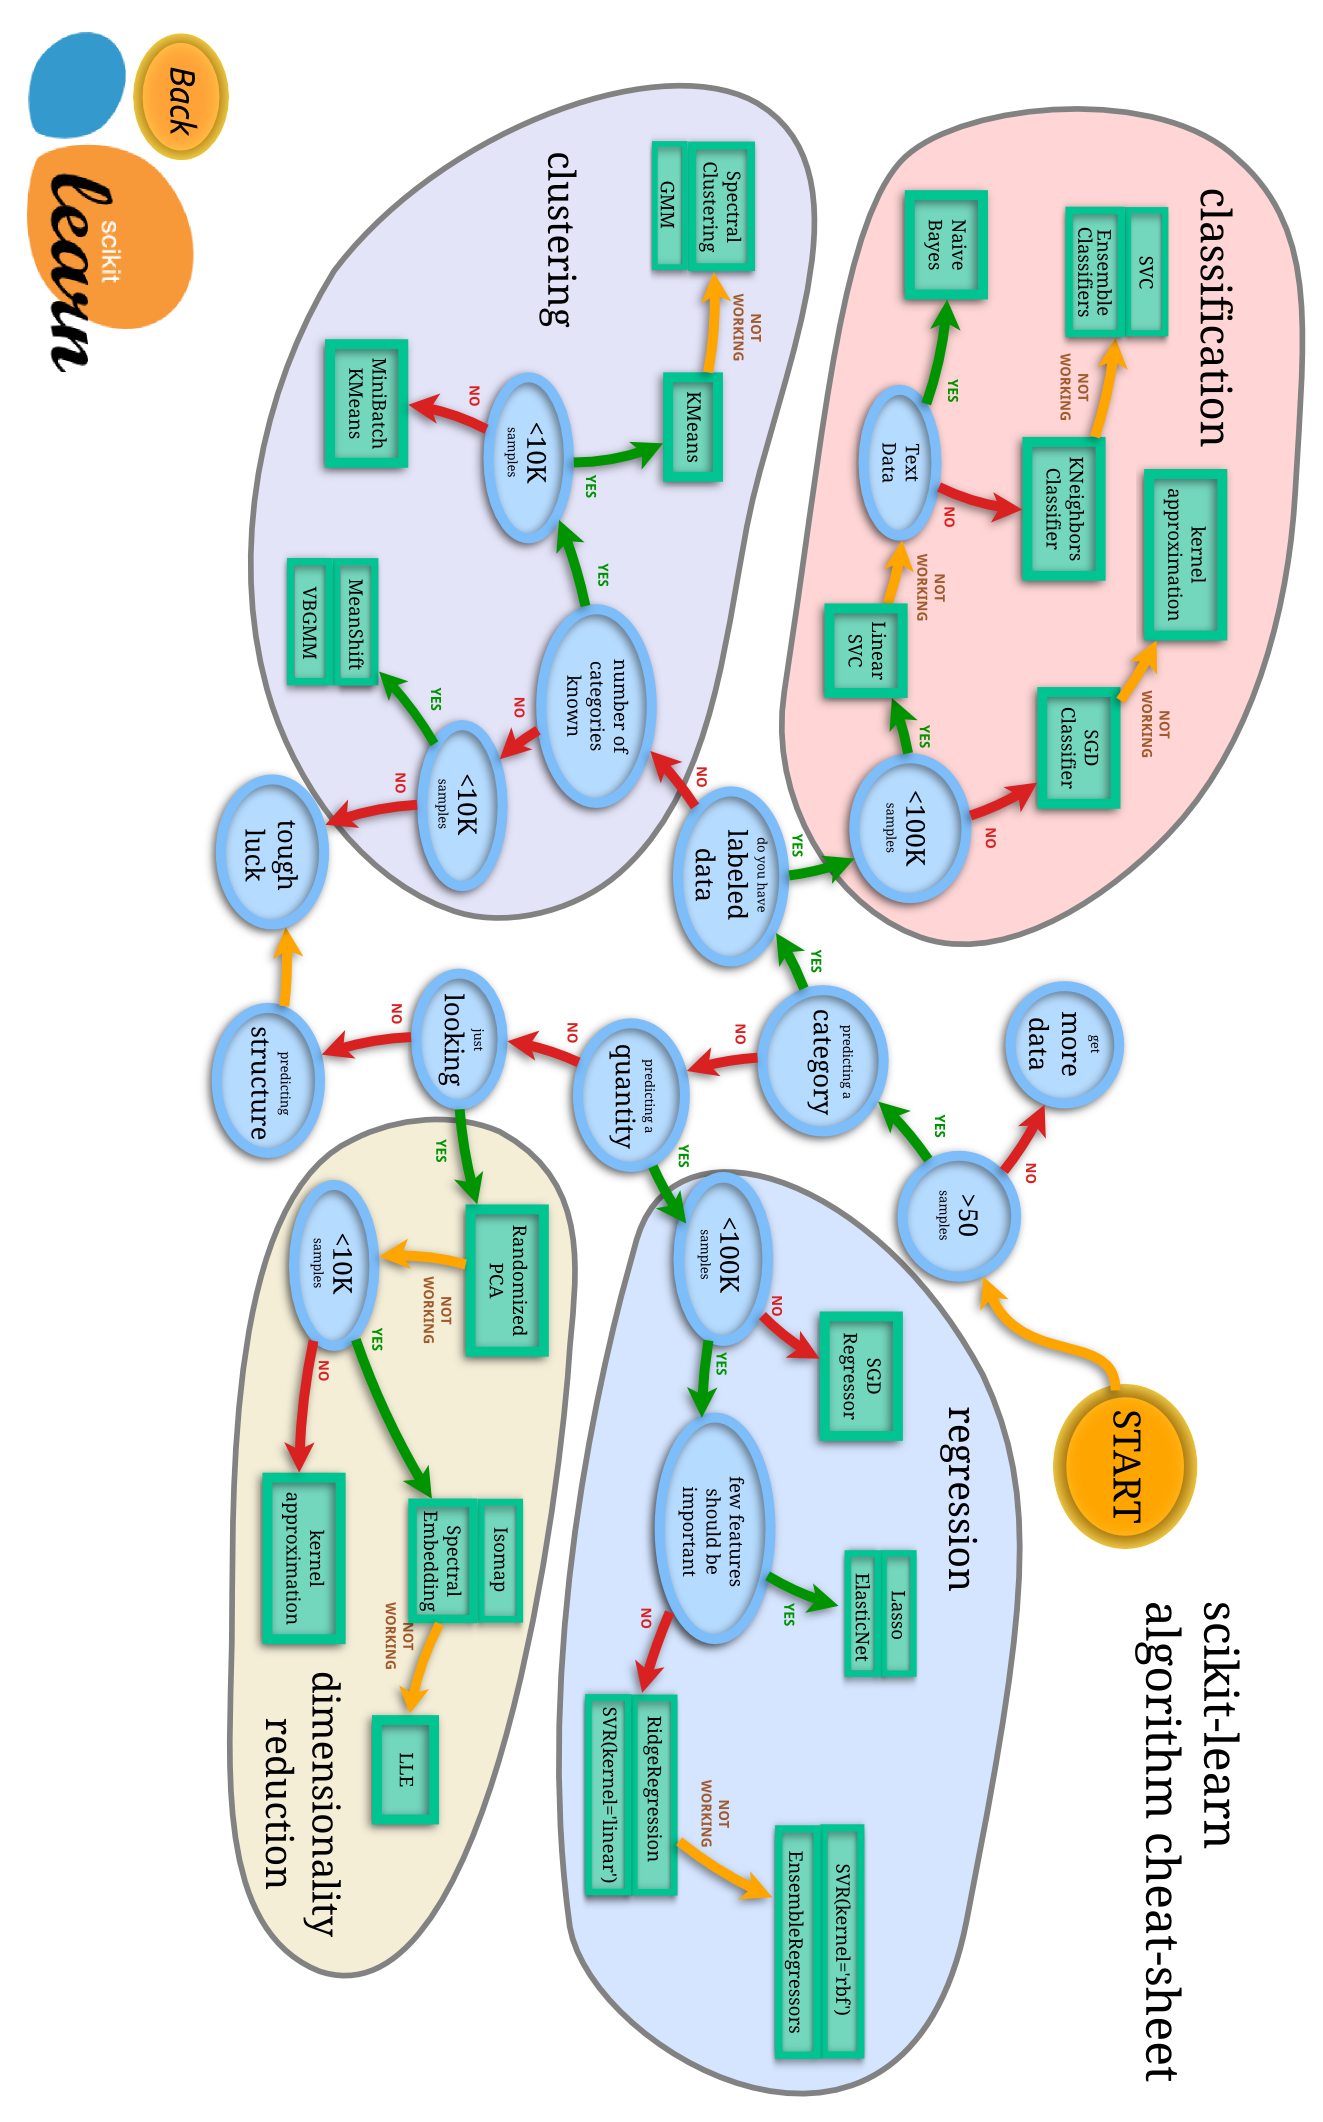
\includegraphics[width=0.645\textwidth]{ml_map}
	\caption[Choosing the right estimator]{Choosing the right estimator \cite{Scikitlearn.org2016i}.}
	\label{fig:ml_map}
\end{figure}

\clearpage
\section{Quick installation guide for Windows x64}
\label{app:installation_windows}
Since Python is much more adapted to *nix systems then Windows, I decided to write a short guide on how to install Python 3.5 and Scikit-learn on Windows. 
This guide is provided as-is, and I make no guarantees that this will result in a functioning installation, but it should at least reduce the problems. 
A presumption here is that the operative system is Windows x64 (if you have x86, you can ignore all the x64 settings).
Before installing anything, download the following:
\begin{itemize}
	\item Python: \url{https://www.python.org/downloads/windows/}. \\
	Select the Python version with "Windows x86-64" in its name.
	\item CygWin: \url{https://cygwin.com/}
	\item MinGW: \url{http://www.mingw.org/}
	\item MySQL connector for Python (Git; only needed for running this project): \\
	\url{https://github.com/mysql/mysql-connector-python}.
	\item x64 version of Numpy and Scipy \cite{Codementor.io2015,Gehrcke2015}: \\ 
	\url{http://www.lfd.uci.edu/~gohlke/pythonlibs/}. \\ 
	The latest available versions at the time of writing is "\emph{numpy-1.11.1rc1+mkl-cp35-cp35m-win\_amd64.whl}" and "\emph{scipy-0.17.1-cp35-cp35m-win\_amd64.whl}".
	\item Scikit-learn (Git): \url{https://github.com/scikit-learn/scikit-learn}
	\item If you do not have a version of Microsoft Visual Studio installed, you need to install Visual Studio 2013 or newer (because compiler requires it)\footnote{
		"vcvarsall.bat needed for python to compile missing from visual studio 2015": \\
		\url{http://stackoverflow.com/q/33323172}
	}.
\end{itemize}


\begin{enumerate}
	\item Install Python, update pip, and install these packages: \\
	\emph{pip install -U bs4 pandas nltk matplotlib cython nose nosetests}
	\item Install MinGW.
	 Thereafter select "mingw32-base" under "MinGW Base System".
	In addition, under "MinGW Base System", select all belonging to Class "bin" and "dll"
	\item Install CygWin. 
	During installation, you will be asked what you want to install. 
	Select all entries that contains "gcc", "mingw64", "make", "automake", "lapack" and "openblas".
	The GCC-compilers are used in combination with MinGW, because Scikit-learn needs Fortran, Lapack and OpenBlas for \emph{make} to succeed.
	\item Change to folder with the x64 version of Numpy and Scipy, and install them~\cite{Codementor.io2015,Gehrcke2015}: \\
	\emph{pip install "numpy-1.11.1rc1+mkl-cp35-cp35m-win\_amd64.whl"} \\
	Verify installation: 1. \emph{python}, 2. \emph{import numpy}, 3. \emph{numpy.\_\_version\_\_}. \\
	\emph{pip install "scipy-0.17.1-cp35-cp35m-win\_amd64.whl"} and verify using the same steps, swapping numpy with scipy.
	\item Start CygWin (run as administrator), change to directory containing Scikit-learn and run the following commands: \\
	\emph{python setup.py build}  and \emph{python setup.py install}.
\end{enumerate}


% backup of various created tables

\begin{comment}
% potentially flip this, and this as a Score X feature (since all kernel values were the same)
% something like "Comparison ..., with Kernel = RBF, Gamma = gamma and C = c
% and the table having features as rows, and score X unprocessed as column
\begin{table}[tbp]
\centering
\begin{tabular}{| c | c | c | c | c | c | c | c |}
\hline
~ 					& Code sample	& Numerical		& Hexadecimal	& Homework		& Link 		& Tags	\\ \hline
Score 				& 0.783			& 0.796			& 0.793			& 0.794			& 0.795 	& 0.757	\\ \hline
C					& 1000			& 1000			& 1000			& 1000			& 1000 		& 1000	\\ \hline
Gamma ($\gamma$)	& 0.001			& 0.001			& 0.001			& 0.001			& 0.001 	& 0.001	\\ \hline
Kernel				& RBF			& RBF			& RBF			& RBF			& RBF 		& RBF	\\ \hline
\end{tabular}
\caption{Comparison of raw data set (unprocessed) and singular feature detectors}
%\label{tab:singular_feature_detector_so2}
\end{table}
\end{comment}

\begin{comment}
\begin{table}[tbp]
\centering
\begin{tabular}{| c | c | c | c | c |}
\hline
~				& Votes < 0			& Votes = 0			& Votes > 0		& All			\\ \hline
Amount			& 659,955			& 5,256,105			& 5,286,971		& 11,203,031	\\ \hline
Oldest			& 06.08.2008		& 06.08.2008		& 31.07.2008	& 31.07.2008 	\\ \hline
Newest			& 06.03.2016		& 06.03.2016		& 06.03.2016	& 06.03.2016	\\ \hline
Vote (lowest)	& -147				& 0					& 1				& -147	 		\\ \hline
Vote (highest)	& -1				& 0					& 13845			& 13845	 		\\ \hline
\end{tabular}
\caption{Overview of the Stack Overflow dataset.}
%\label{tab:dataset_overview_so2}
\end{table}
\end{comment}

\begin{comment}
Amount of features before anything was done to the text: 69766 - CountVectorizer(analyzer='word') - \%
Amount of features after adding stop word (English): 69462 - CountVectorizer(analyzer='word', stop\_words="english") - \%
Amount of features after removing code samples, hexadecimals and numeric values: 27624 - \%
Amount of features after setting minimum document frequency: 440 - CountVectorizer(analyzer='word', min\_df=0.01, stop_words='english') - \%


Originally tagged questions as good/bad, but then switched to +/-1 due to considering switching to LibSVM.
\end{comment}
